\section{Macroscopic traffic trends}
\label{section:malawi:macro}

\begin{figure}
  \centering
  \begin{subfigure}[b]{1.0\linewidth}
  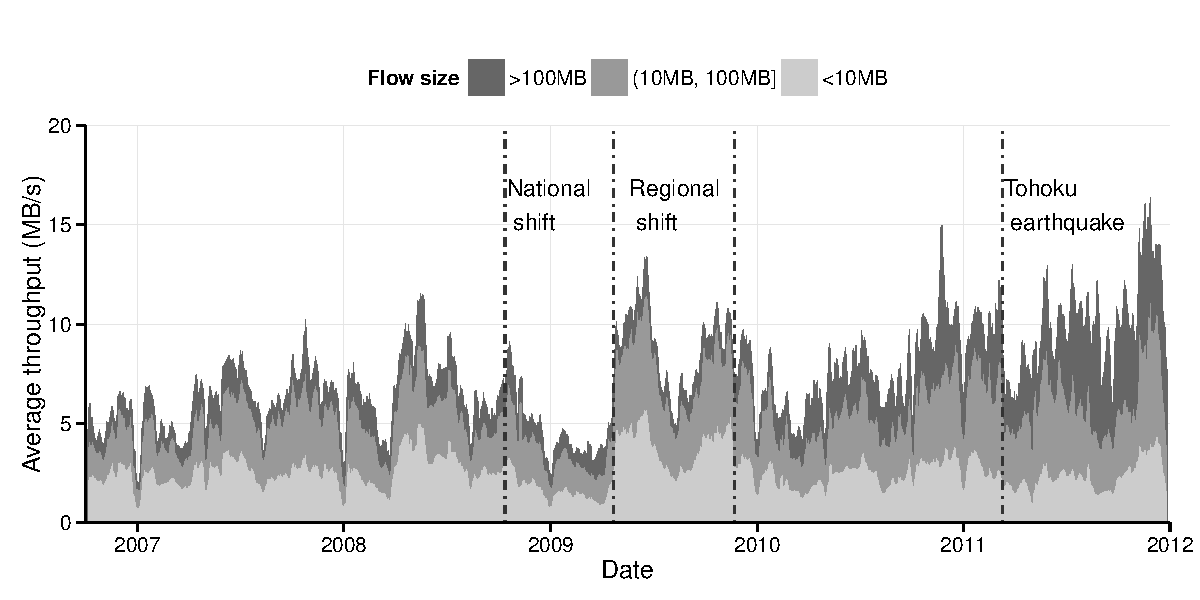
\includegraphics[width=0.9\textwidth]{figures/malawi/tputout}\\
  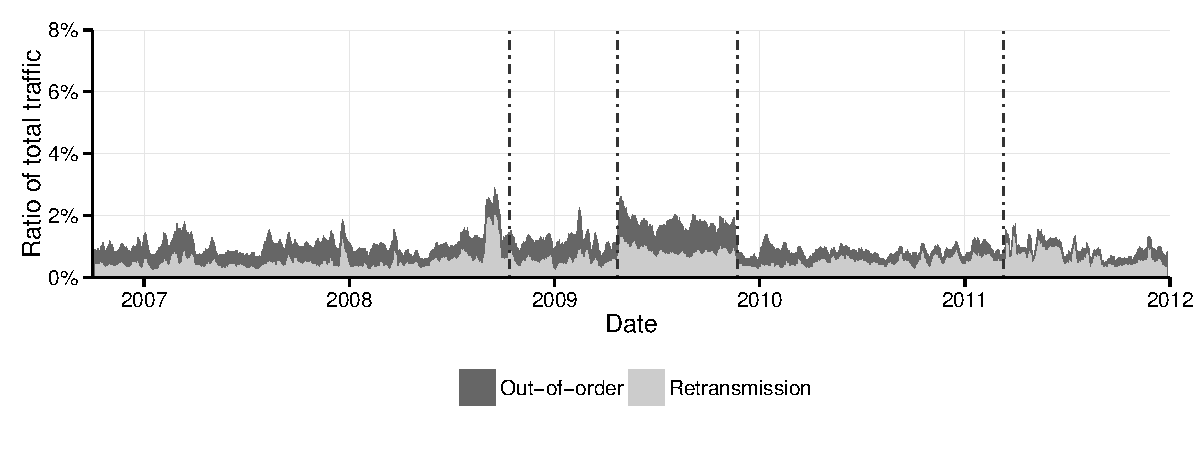
\includegraphics[width=0.9\textwidth]{figures/malawi/lossesout}
  \caption{Inbound traffic\label{fig:MAWIin}}
  \end{subfigure}
  \begin{subfigure}[b]{1.0\linewidth}
  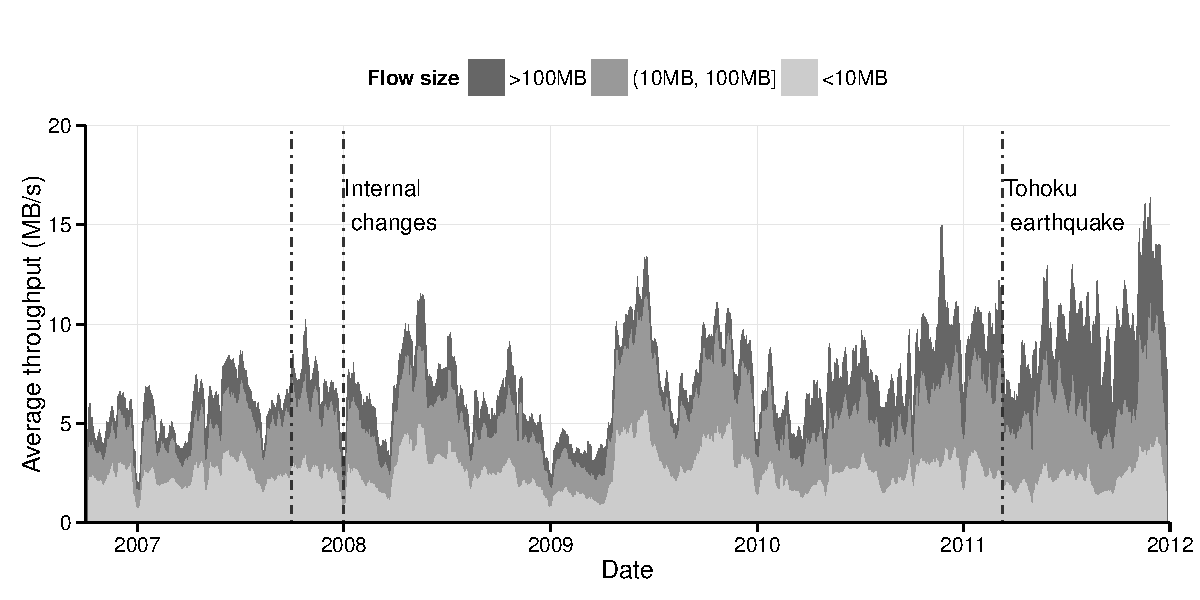
\includegraphics[width=0.9\textwidth]{figures/malawi/tputin}\\
  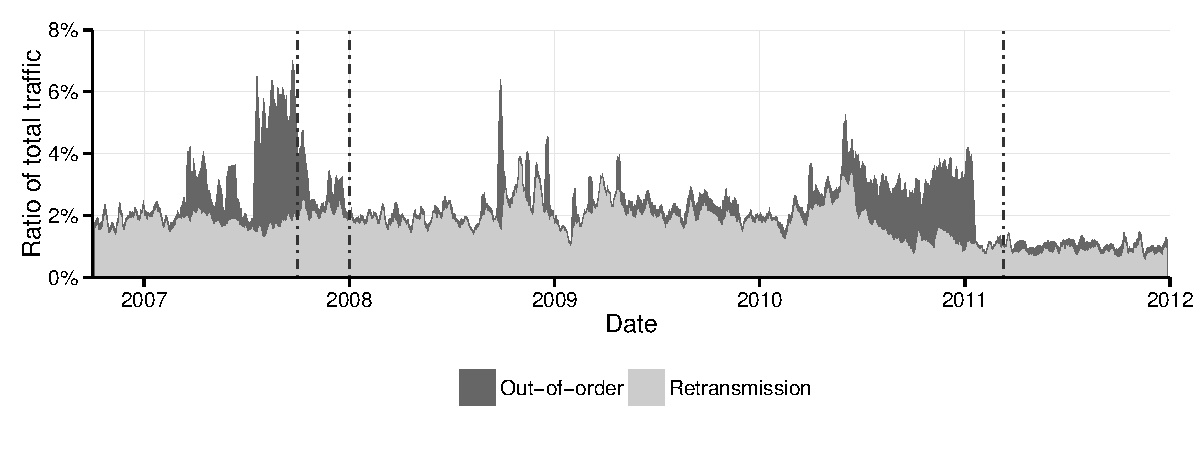
\includegraphics[width=0.9\textwidth]{figures/malawi/lossesin}
  \caption{Outbound traffic\label{fig:MAWIout}}
  \end{subfigure}
  \caption{Longitudinal evolution of average throughput and loss for the \acs{MAWI} dataset.}\label{fig:MAWI}
\end{figure}

Over a five year period, changes in routing and application popularity have continually redefined the nature of traffic under observation.
This section provides a macroscopic view of these shifting trends. 
Figure \ref{fig:MAWI} displays the average throughput and loss ratio for traffic in either direction, calculated for TCP traffic only, smoothed on a weekly basis. 

For inbound traffic, shown in figure \ref{fig:MAWIin}, two routing changes internal to WIDE had significant impact on overall traffic, and are consequently highlighted.
The first, performed towards the end of 2008, diverted most of the inbound traffic from \emph{national} sources away from the monitored transit link, resulting in a reduction of traffic.
This event was preceded by increased congestion downstream from the monitoring point.
The second, in early 2009, saw a significant increase in \emph{regional} traffic from Asian neighbours, and was reverted approximately six months later. 
During this period aggregate end-to-end loss rates increased as a result.
While this is mostly due to the higher proportion of upstream congestion for traffic from Taiwan and China in particular, most traffic was adversely affected by the increased utilisation, suggesting that the transit link itself may have been a bottleneck during this period.
Finally, the impact of the Tohuku earthquake resulted in a noticeable break in demand coinciding with the start of the Japanese fiscal year in April, in which traffic traditionally ramps up.

For reference, relevant metrics for outbound traffic are also shown in figure \ref{fig:MAWIout}.
Compared to inbound traffic, outbound traffic is subject to higher rates of out-of-sequence packets.
The proportion of out-of-order packets in particular is large for extended periods of time at the end of both 2007 and 2011, ending abruptly.
This either suggests that the internal network was congested and eventually upgraded, or that load-balancing mechanisms leading to increased network reordering were employed and then decommissioned.
The higher rate of retransmissions on the other hand is largely related to the geographic differences between traffic sources and traffic sinks in the \acs{MAWI} dataset.

\subsection{Geographic distribution}
\label{section:malawi:geo}

This skew in the location of end points is apparent in table \ref{table:dest}, which highlights the geographic distribution of both inbound and outbound traffic for the observed time period.

The majority of traffic flows to and from the United States, which has increased its share of bandwidth in either direction over the past five years. 
The proportion of traffic flowing from the United States is particularly high, accounting for almost 70\% of inbound traffic in 2011. 
While this may foreshadow an increased concentration of traffic from the United States, it should primarily be viewed as a reflection of routing policy, with regional traffic being diverted to alternate routes as Japan became increasingly interconnected to its neighbours.
Of particular importance is the routing change at the end of 2008, which resulted in a sharp drop in inbound traffic from within Japan, as highlighted in figure \ref{fig:MAWIin}.
This event had a profound influence in shaping not only the distribution of traffic, but also delay as shall be observed in section \ref{section:malawi:delay}.

Further geographic shifts in the inbound direction are apparent when breaking down US traffic by state.
The proportion of traffic originating from California has decreased over time, dropping from 55\% of total US traffic in 2007 to only 35\% in 2011.
In its place, a larger set of states have emerged as content providers, with New Jersey, Florida and Virginia contributing over a quarter of all traffic originating within the US by 2011.

\begin{table}\footnotesize\centering
    \begin{tabular}{  
@{}
$>{\scshape}p{3.0cm}
^r
^r
^r
^r
^r@{\hskip 1.0cm}
^r
^r
^r
^r
^r
@{}
}
\toprule
\rowstyle{\scshape\bfseries}
\multirow{2}{*}{\parbox[][0.7cm][b]{3.0cm}{Country}} & 
\multicolumn{5}{c}{\scshape\bfseries{Outbound traffic (\%)\hspace*{0.45cm}}} & 
\multicolumn{5}{c}{\scshape\bfseries{Inbound traffic (\%)}} \\
\cmidrule(r{1.0cm}){2-6} \cmidrule{7-11}
\addlinespace[-0.6em] \rowstyle{\scriptsize\scshape}
 & 2007 & 2008 & 2009 & 2010 & 2011 & 2007 & 2008 & 2009 & 2010 & 2011 \\
\midrule

        United States & 27.3 & 31.3 & 29.3 & 36.4 & 35.7 & 45.7 & 41.5 & 53.3 & 65.1 & 67.1
\\
        \scriptsize{ California } & \scriptsize{ 39.0 } & \scriptsize{ 61.8 } & \scriptsize{ 63.5 } & \scriptsize{ 53.8 } & \scriptsize{ 50.6 } & \scriptsize{ 55.7 } & \scriptsize{ 47.9 } & \scriptsize{ 46.7 } & \scriptsize{ 24.9 } & \scriptsize{ 34.9 }\\\scriptsize{ Texas } & \scriptsize{  5.8 } & \scriptsize{  4.3 } & \scriptsize{  4.1 } & \scriptsize{  2.4 } & \scriptsize{ 13.9 } & \scriptsize{  7.0 } & \scriptsize{ 12.0 } & \scriptsize{  5.8 } & \scriptsize{  7.1 } & \scriptsize{  5.6 }\\\scriptsize{ Colorado } & \scriptsize{  1.9 } & \scriptsize{  1.2 } & \scriptsize{  0.6 } & \scriptsize{  8.5 } & \scriptsize{  2.8 } & \scriptsize{  4.9 } & \scriptsize{  6.0 } & \scriptsize{  5.9 } & \scriptsize{  9.7 } & \scriptsize{  5.8 }\\\scriptsize{ Virginia } & \scriptsize{  1.9 } & \scriptsize{  1.0 } & \scriptsize{  0.8 } & \scriptsize{  0.4 } & \scriptsize{  0.6 } & \scriptsize{  1.2 } & \scriptsize{  3.0 } & \scriptsize{ 14.1 } & \scriptsize{ 13.1 } & \scriptsize{  8.3 }\\\scriptsize{ Washington } & \scriptsize{  4.0 } & \scriptsize{  2.9 } & \scriptsize{  3.5 } & \scriptsize{  6.1 } & \scriptsize{  6.6 } & \scriptsize{  0.9 } & \scriptsize{  5.7 } & \scriptsize{  3.5 } & \scriptsize{  3.0 } & \scriptsize{  2.0 }\\\scriptsize{ New Jersey } & \scriptsize{  2.8 } & \scriptsize{  1.5 } & \scriptsize{  0.7 } & \scriptsize{  1.1 } & \scriptsize{  1.9 } & \scriptsize{  1.0 } & \scriptsize{  1.8 } & \scriptsize{  1.6 } & \scriptsize{  4.9 } & \scriptsize{ 13.6 }\\\scriptsize{ Massachusetts } & \scriptsize{  1.6 } & \scriptsize{  1.1 } & \scriptsize{  0.9 } & \scriptsize{  6.1 } & \scriptsize{  4.9 } & \scriptsize{  5.4 } & \scriptsize{  2.1 } & \scriptsize{  1.8 } & \scriptsize{  1.6 } & \scriptsize{  2.0 }\\\scriptsize{ Florida } & \scriptsize{  3.1 } & \scriptsize{  2.3 } & \scriptsize{  1.3 } & \scriptsize{  1.1 } & \scriptsize{  0.9 } & \scriptsize{  1.0 } & \scriptsize{  0.4 } & \scriptsize{  0.4 } & \scriptsize{  8.5 } & \scriptsize{  7.9 }
\\
        Japan & 11.6 & 15.4 & 17.7 & 16.7 & 16.1 & 33.8 & 32.2 &  7.3 & 8.1 & 11.5\\China &  7.9 & 20.5 & 17.8 & 10.3 &  5.9 &  2.5 &  5.3 &  6.3 & 4.6 &  3.1\\Korea, Republic of &  5.3 &  1.3 &  2.1 &  7.8 & 23.8 &  4.7 &  5.1 &  3.2 & 1.1 &  0.5\\Germany &  2.2 &  1.7 &  1.6 &  1.0 &  0.6 &  3.0 &  6.1 &  5.3 & 5.5 &  1.4\\Taiwan &  2.7 &  1.3 &  4.0 &  3.6 &  2.7 &  0.8 &  0.9 & 10.9 & 0.9 &  0.4\\Netherlands &  0.4 &  0.4 &  0.5 &  0.3 &  0.4 &  0.9 &  1.0 &  4.1 & 6.2 &  6.9\\India &  2.8 &  3.3 &  4.8 &  3.3 &  2.0 &  0.3 &  0.1 &  0.0 & 0.2 &  0.0\\France &  1.2 &  1.1 &  0.9 &  0.9 &  0.9 &  1.6 &  1.2 &  2.6 & 3.4 &  1.7\\United Kingdom &  1.1 &  1.0 &  1.0 &  0.9 &  0.7 &  2.5 &  2.2 &  1.6 & 1.3 &  1.3
\\
    \bottomrule
    \end{tabular}
  \caption{Percentage of inbound and outbound traffic by country\label{table:dest}. U.S. state values are relative to total national traffic.}
\end{table}
%tip

In the outbound direction, the geographic distribution of traffic is less skewed, with a greater proportion of traffic flowing towards Japan and China in particular. 
Traffic to the Republic of Korea progressively increases from 2010 onwards due to successive routing changes.
Combined with the drop in traffic towards China, this accounts for much of the drop in aggregate loss rates since 2010, as observable in figure \ref{fig:MAWIout}.
European destinations overall have a small proportion of outgoing traffic, which appears to be shrinking over time. 
The most significant factor for the discrepancy between inbound and outbound traffic for Europe as a whole is the time zone difference, as traffic is measured at 05:00\acs{GMT}. 
This however does not account for why outbound traffic overall has been falling. 
Since most outbound traffic towards Europe at the time of measurement is likely to be scheduled transfers with no human intervention, a plausible explanation for this trend is the gradual shift away from file-sharing using peer-to-peer applications. 
This is further corroborated by the rise of hosting solutions which facilitate file-sharing, as shall become evident when analyzing the breakdown of traffic by \ac{AS}.

\subsection{\acs{AS}-level distribution}
\label{section:malawi:as}

\begin{figure}
    \centering
    \begin{subfigure}[b]{0.5\linewidth}
        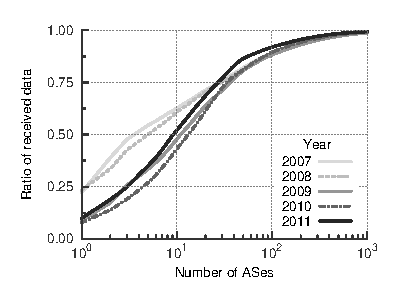
\includegraphics{figures/malawi/asn_cdf_in}
        \caption{\label{fig:asn_cdf_in}}
    \end{subfigure}%
    \begin{subfigure}[b]{0.5\linewidth}
        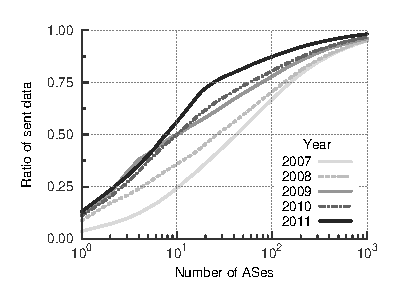
\includegraphics{figures/malawi/asn_cdf_out}
        \caption{\label{fig:asn_cdf_out}}
    \end{subfigure}%
    \caption[\acs{CDF} of traffic by \acs{AS}]{\acs{CDF} of (\subref{fig:asn_cdf_in}) inbound and (\subref{fig:asn_cdf_out}) outbound traffic by \acs{AS}.\label{fig:asn_cdf}}
\end{figure}

\begin{table}\scriptsize\centering
    \begin{subtable}[b]{.33\linewidth}
    \begin{tabular}{
@{}
$>{\raggedleft}p{0.6cm}
^>{\scshape}p{2.25cm}
^>{\raggedleft\arraybackslash}p{0.6cm}
@{}
}
\toprule
\rowstyle{\scshape\bfseries}
\acs{ASN} & \acs{AS} name &
\% \\
\midrule

    2914 & Ntt & 29.92 \\36561 & Youtube & 15.89 \\15169 & Google & 3.80 \\22822 & Limelight & 3.70 \\174 & Cogent & 3.03 \\9318 & Hanaro & 2.46 \\3356 & Level 3 & 1.97 \\20940 & Akamai & 1.53 \\19166 & Acronoc & 1.47 \\30212 & DTI Services & 1.05 \\

    \bottomrule
    \end{tabular}
    \caption{2007}
    \end{subtable}%
    \begin{subtable}[b]{.33\linewidth}
    \begin{tabular}{
@{}
$>{\raggedleft}p{0.6cm}
^>{\scshape}p{2.25cm}
^>{\raggedleft\arraybackslash}p{0.6cm}
@{}
}
\toprule
\rowstyle{\scshape\bfseries}
\acs{ASN} & \acs{AS} name &
\% \\
\midrule

    3462 & HiNet & 9.78 \\15169 & Google & 8.64 \\43515 & Google (Youtube) & 7.92 \\2914 & Ntt & 5.89 \\46742 & Carpathia (LAX) & 4.17 \\4766 & Korea Telecom & 2.74 \\4134 & China Telecom & 2.62 \\3356 & Level 3 & 2.14 \\4837 & China Unicom & 2.10 \\36561 & Youtube & 1.98 \\

    \bottomrule
    \end{tabular}
    \caption{2009}
    \end{subtable}
    \begin{subtable}[b]{.33\linewidth}
    \begin{tabular}{
@{}
$>{\raggedleft}p{0.6cm}
^>{\scshape}p{2.25cm}
^>{\raggedleft\arraybackslash}p{0.6cm}
@{}
}
\toprule
\rowstyle{\scshape\bfseries}
\acs{ASN} & \acs{AS} name &
\% \\
\midrule

    2914 & Ntt & 10.79 \\20473 & Choopa & 8.86 \\43515 & Google (Youtube) & 8.65 \\35415 & Webazilla & 6.01 \\40824 & WZ Comm. & 4.79 \\15169 & Google & 4.66 \\40263 & FC2 & 3.61 \\30212 & DTI Services & 2.68 \\16265 & LeaseWeb & 2.56 \\29748 & Carpathia (VA) & 2.05 \\

    \bottomrule
    \end{tabular}
    \caption{2011}
    \end{subtable}
  \caption[Top 10 \acp{AS} for inbound traffic by year.]{Top 10 \acp{AS} for inbound traffic by year.\label{table:topASin}}
\end{table}

\begin{table}\scriptsize\centering
    \begin{subtable}[b]{.33\linewidth}
    \begin{tabular}{
@{}
$>{\raggedleft}p{0.6cm}
^>{\scshape}p{2.25cm}
^>{\raggedleft\arraybackslash}p{0.6cm}
@{}
}
\toprule
\rowstyle{\scshape\bfseries}
\acs{ASN} & \acs{AS} name &
\% \\
\midrule

    15169 & Google & 3.94 \\7132 & Sbis AT\&T & 3.23 \\4134 & China Telecom & 3.14 \\10013 & FreeBit & 2.91 \\4788 & TM Net & 2.37 \\9318 & Hanaro & 2.21 \\9595 & Xephion Ntt & 2.09 \\9304 & Hutchison AS & 2.00 \\2914 & Ntt & 1.90 \\4837 & China Unicom & 1.72 \\

    \bottomrule
    \end{tabular}
    \caption{2007}
    \end{subtable}%
    \begin{subtable}[b]{.33\linewidth}
    \begin{tabular}{
@{}
$>{\raggedleft}p{0.6cm}
^>{\scshape}p{2.25cm}
^>{\raggedleft\arraybackslash}p{0.6cm}
@{}
}
\toprule
\rowstyle{\scshape\bfseries}
\acs{ASN} & \acs{AS} name &
\% \\
\midrule

    15169 & Google & 11.55 \\2510 & Infoweb & 11.32 \\4134 & China Telecom & 9.10 \\2518 & Biglobe NEC & 6.00 \\3462 & HiNet & 3.78 \\4837 & China Unicom & 3.01 \\14778 & Inktomi & 2.04 \\7132 & Sbis AT\&T & 1.51 \\36647 & Yahoo & 1.14 \\24560 & Airtel & 1.13 \\

    \bottomrule
    \end{tabular}
    \caption{2009}
    \end{subtable}
    \begin{subtable}[b]{.33\linewidth}
    \begin{tabular}{
@{}
$>{\raggedleft}p{0.6cm}
^>{\scshape}p{2.25cm}
^>{\raggedleft\arraybackslash}p{0.6cm}
@{}
}
\toprule
\rowstyle{\scshape\bfseries}
\acs{ASN} & \acs{AS} name &
\% \\
\midrule

    4766 & Korea Telecom & 11.39 \\15169 & Google & 8.66 \\2510 & Infoweb & 5.93 \\3549 & Global Crossing & 5.38 \\9318 & Hanaro & 4.76 \\36647 & Yahoo & 4.63 \\2518 & Biglobe NEC & 4.23 \\46179 & Mediafire & 3.42 \\17858 & Konyang Univ. & 2.77 \\3462 & HiNet & 2.68 \\

    \bottomrule
    \end{tabular}
    \caption{2011}
    \end{subtable}
  \caption[Top 10 \acp{AS} for outbound traffic by year.]{Top 10 \acp{AS} for outbound traffic by year.\label{table:topASout}}
\end{table}

%tip
It has been widely noted that interdomain traffic has significantly changed over the past decade, with an increasing proportion of traffic flowing to and from a dwindling set of both large content providers and consumer networks. 
Such traffic consolidation is most apparent at the AS level, where a direct mapping to a commercial entity is forthcoming.

In the inbound direction traffic has remained consistently concentrated in the top 100 \acp{AS} accounting for approximately 90\% of all data received, as shown by the cumulative distribution of inbound traffic by \acs{AS} in \ref{fig:asn_cdf_in}.
There is a visible drop in concentration amongst the top \acp{AS} between 2008 and 2009 as a wide range of Japanese prefixes were rerouted through a different ingress.
This shift is clarified in table \ref{table:topASin}, which lists the top ten \acp{AS} by received data for 2007, 2009 and 2011.
While in 2007 traffic was already consolidated across a small set of \acp{AS}, a significant portion of transit traffic was still Asian: most traffic from \acs{NTT} and Limelight originated from within Japan. 
Such traffic has gradually been pushed away from transit by 2011.
Large carriers such as Cogent, Level3, Hanaro, China Telecom have also seen their importance diluted by \acp{AS} known to harbour \ac{OCH} services such as Choopa, Webazilla, WZ Communications, Carpathia and LeaseWeb.
Many of the hosted websites facilitate the distribution of copyrighted content, and as such are not capable of growing large enough to expand beyond hosted infrastructure without risking prosecution.

For outbound traffic, shown in figure \ref{fig:asn_cdf_out}, consolidation has been much more perceptible. 
For the top 10 \acp{AS} alone, the proportion of traffic has more than doubled between 2007 and 2011. 
By 2011, the distribution of traffic amongst \acp{AS} for inbound and outbound traffic bears a striking similarity but the nature of this concentration is markedly different, as made apparent by table \ref{table:topASout}.
Despite the increased importance of content providers and \ac{OCH} services such as Google, Yahoo and Mediafire, significant portions of outgoing traffic continue to flow toward eyeball \acp{ISP} such as Korea Telecom, Infoweb, Global Crossing and Hanaro.

% overall summary: content consolidation, delay, etc
Overall, the observed traffic patterns match the insights provided by Labovitz et al.\ on the changing nature of interdomain traffic in \cite{Labovitz:2010p175}, but highlight that such trends have occurred at different paces depending on the direction of traffic. 
Inbound traffic showed strong signs of concentration as early as 2007, whereas outbound traffic has only become dominated by large consumer networks and regional providers more recently.
The implications for transit traffic from an Asian perspective is less intuitive: with the increased adoption of \acp{CDN} and \acp{IXP}, more transit traffic is being retrieved from further away as content in the United States shifts eastward.

\subsection{Delay}
\label{section:malawi:delay}
 
While understanding where traffic flows to and from is of great value at an operational, commercial and often political level, it portrays a small part of a wider picture. 
For end-users it is of less concern where content is being retrieved from or routed through compared to how long it takes.

\begin{figure}
    \centering
    \begin{subfigure}[b]{0.5\linewidth}
        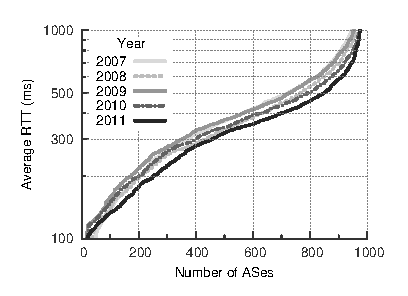
\includegraphics{figures/malawi/rtt_cdf_in}
        \caption{\label{fig:rtt_cdf_in}}
    \end{subfigure}%
    \begin{subfigure}[b]{0.5\linewidth}
        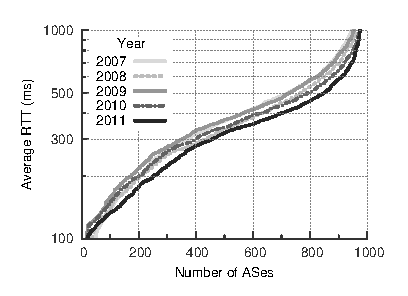
\includegraphics{figures/malawi/rtt_cdf_out}
        \caption{\label{fig:rtt_cdf_out}}
    \end{subfigure}%
    \caption[\acs{CDF} of mean \acs{RTT} by \acs{AS}]{\acs{CDF} of mean \acs{RTT} by \acs{AS} for (\subref{fig:rtt_cdf_in}) inbound and (\subref{fig:rtt_cdf_out}) outbound traffic. \label{fig:rtt_cdf}}
\end{figure}

Intuitively delay should decrease over time as the Internet becomes more interconnected, resulting in less path stretch, and access technology improves, cutting down queuing delay in particular.
This is partially confirmed by figure \ref{fig:rtt_cdf}, which displays the mean delay distribution for traffic in either direction.
Given the long-tailed nature of traffic, many \acp{AS} have a limited number of \ac{RTT} samples.
As such, only the thousand most significant \acp{AS} in either direction are used to plot the respective \acs{CDF}.

As with traffic distributions, the plots once again illustrate the same overall trend in subtly different patterns. 
While latency has dropped across the board, the rate of improvement is markedly different. 
Taking the median of both plots as a reference point, delay has dropped by 20$ms$ between 2009 and 2011 for inbound traffic, nearly half the equivalent decrease for outbound traffic.
The absolute values in both cases are still disparate: over 90\% of \acp{AS} are reached within a round trip time of approximately 400$ms$ when ranked by inbound traffic, whereas the equivalent value for outbound traffic is almost 200$ms$ higher. 
For inbound traffic the average \ac{RTT} is low enough that geographical properties are clearly visible. 
A first plateau close to 100$ms$ is apparent for traffic to the American west coast, while traffic to European destinations is clustered close to 250$ms$. 
Tellingly, this second plateau seems to be receding.
When taken in conjunction with the geographic distribution of traffic presented in table \ref{table:dest} this seems to confirm the reduction in the number of sources within Europe. 

A pertinent question at this point is in trying to understand how delay relates to traffic volumes. 
Given the different nature of stakeholders monopolizing traffic at either end of the spectrum, what can be said about the evolution of delay in either case? 
Figure \ref{fig:rtt_wcdf} plots the cumulative distribution of the average \ac{RTT} weighted by the respective volume of traffic.
In interpreting such plots one should keep in mind that they provide a rough indicator of the average delay to be expected if one were to sample a packet belonging to the top $N$ sources or destinations. 
As $N$ increases, the resulting value approaches the average RTT for all traffic in a given direction.

\begin{figure}
    \centering
    \begin{subfigure}[b]{0.5\linewidth}
        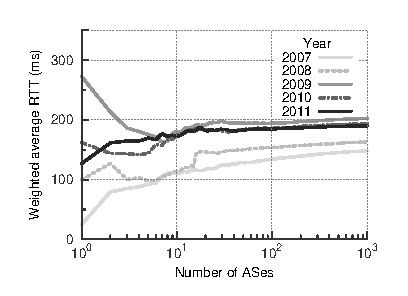
\includegraphics{figures/malawi/rtt_wcdf_in}
        \caption{\label{fig:rtt_wcdf_in}}
    \end{subfigure}%
    \begin{subfigure}[b]{0.5\linewidth}
        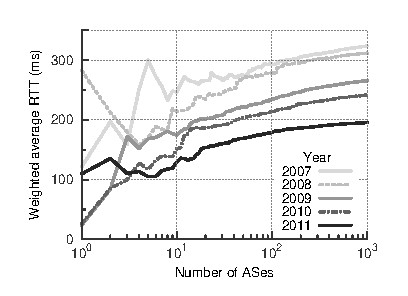
\includegraphics{figures/malawi/rtt_wcdf_out}
        \caption{\label{fig:rtt_wcdf_out}}
    \end{subfigure}%
    \caption[\acs{CDF} of weighted \acs{RTT} by \acs{AS}.]{\acs{CDF} of weighted \acs{RTT} by \acs{AS} for (\subref{fig:rtt_wcdf_in}) inbound and (\subref{fig:rtt_wcdf_out}) outbound traffic. \label{fig:rtt_wcdf}}
\end{figure}

Inbound traffic by \ac{AS} highlights an expected rise in delay between 2008 and 2009, as both \acs{NTT} and Limelight are replaced by more distant sources. 
However, from 2009 onwards the overall delay remains remarkably stable. 
While the cumulative distribution function of \ac{RTT} shows improvement in delay at the tail, this results in very little improvement overall as traffic is dominated by a handful of entities.

Two explanations emerge for this behaviour. 
The first stems from the changing nature of the traffic being sampled. 
While functionally \acs{NTT} represents the same entity over time, the traffic under observation is very different. 
The local view of traffic has been stretched further afield as data has been increasingly exchanged over peering links, particularly at a national level.
This is particularly noticeable in figure \ref{fig:rtt_wcdf_in}, where the average delay towards \acs{NTT}, the most significant \ac{AS} for inbound traffic in both 2007 and 2011, increased by approximately 100$ms$.
This does not represent a degradation in quality of service, but rather a change in where traffic is flowing from within the \acs{AS}.

A further reason relates to the placement of content. 
As previously established in table \ref{table:dest}, there appears to be a migration of content away from California. 
\ac{OCH} providers such as Lemuria, based in Florida, Mediafire, based in Texas and District of Columbia and Carpathia, based in Virginia, are all contained within the top 20 \acp{AS} and have shifted traffic further from locations which had traditionally benefited from low latency as viewed from Japan.

Analyzing the outbound traffic seemingly reveals the opposite effect, with the average weighted \ac{RTT} dropping by over 100ms. 
Once more, there is no single reason which accounts for the entirety of this effect. 
In 2007 many of the top destination \acp{AS} were in developing Asian countries, where infrastructure has improved greatly since. 
Improvements in routing to countries such as China and the Republic of Korea have also had a positive net effect. 
This is visible in figure \ref{fig:rtt_comp}, where the average \ac{RTT} aggregated by country is plotted. 
For clarity, countries for which RTT estimates are available for less than 50 days in a year are filtered out. 
Between 2007 and 2009 most Asian and European countries experience significant improvements in \ac{RTT}.
The minor exceptions are typically countries for which delay was already comparatively low.
By 2011, latency to most countries had been reduced below 500$ms$.

\begin{figure}
    \centering
    \begin{subfigure}[b]{0.5\linewidth}
        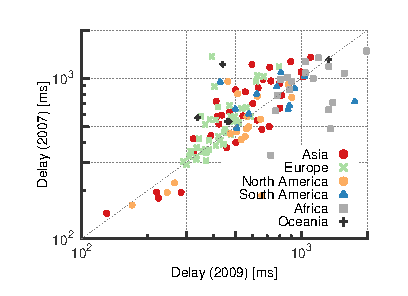
\includegraphics{figures/malawi/rtt_comp_07_09}
        \caption{2007/2009}
    \end{subfigure}%
    \begin{subfigure}[b]{0.5\linewidth}
        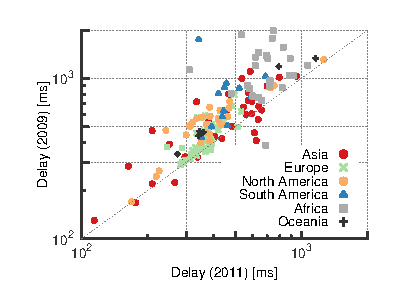
\includegraphics{figures/malawi/rtt_comp_09_11}
        \caption{2009/2011}
    \end{subfigure}%
    \caption{Scatter plot of mean RTT by country grouped by continent.\label{fig:rtt_comp}}
\end{figure}

Finally, many of the very same companies which have had an effect of increasing \ac{RTT} for inbound traffic, such as Mediafire or Ustream.tv, are also amongst the top destinations of traffic. 
It is interesting to note that as of 2011, data travelling from the top 1000 \ac{AS} traffic sources was expected to experience the same latency as data travelling towards the 1000 most popular \ac{AS} traffic destinations. 
In 2007, the value was two times higher for outgoing traffic.
Traffic downstream is moving further away as content is not only placed closer to consumers and bypasses the transit link entirely, but also moves deeper within the United States, whereas traffic upstream has been drawn closer. 

